\section{自然语言关系的主宾语类型搭配研究}
\label{sec:tinf}

TODO: poster里面的图可以放进来!!

%============================================================%

%# -*- coding: utf-8-unix -*-
% !TEX program = xelatex
% !TEX root = ../thesis.tex
% !TEX encoding = UTF-8 Unicode

\subsection{引言}
\label{sec:tinf-intro}
% 1. give a example of ambiguous relation
% 2. talk about selectional preference
% 3. talk about open ie
% Goal: Why we do this work? What's the help of pairwise selectional preference?
% Reverb has high quality

% open ie part
% 1. recent years, open ie system played an important rule

开放式信息抽取(Open Information Extraction)任务的目标是从
从开放领域的文本语料库中挖掘命名实体或概念,并抽取出连接这些实体的
各种不同的自然语言关系。
之所以称为开放式抽取,是因为要挖掘的关系不局限于特定领域
也不基于固定的匹配规则。
学术界中,较为先进的开放式信息抽取系统
\cite{carlson2010toward,fader2011identifying,schmitz2012open,nakashole2012patty}
可以从海量互联网语料库中,以很高的准确率提取百万甚至更高级别数量的关系实例,
($arg_1$, $rel$, $arg_2$)三元组形式,我们将其称为关系三元组。
其中,$rel$为二元关系,
一般表示为短语(词级别描述)或依存语法路径(语法级别描述)。
$arg_1$和$arg_2$是关系的两个参数,即主语和宾语,同样表现为短语形式。


% 4. it's interesting to see the semantic information hidden in these tuples.
开放式信息抽取提供给我们海量关系实例的同时,
我们有兴趣将这些实例进行归纳,寻找更加抽象的语义表示。
我们关注的重点就是这些关系所具有的不同含义。
以关系 ``play in'' 为例,开放式信息抽取系统可以提供
一系列具有($X$, play in, $Y$)形式的三元组。
例如ReVerb系统\cite{fader2011identifying}可抽取出三元组
(Goel Grey, played in, Cabaret)以及(Tom Brady, play in, National Football League)。
%\begin{center}
%$\langle \text{Goel Grey}, played\ in, \text{Cabaret} \rangle$ \\
%$\langle \text{Tom Brady}, play\ in, \text{National Football League} \rangle$
%\end{center}
%本章的目标是通过已有的关系实例,自动推理出
给定某关系已有的三元组实例,我们可以推理出一系列
由类型三元组描述的关系模式,即主宾语类型搭配($t_1$, play in, $t_2$)。
其中$t_1$以及$t_2$为标准化的实体类型,其来源为含有类型定义的知识库,
例如WordNet\cite{miller1995wordnet},%如果还有别的地方提到了WN,那么这里就不要提了
Yago\cite{suchanek2007WWW},Freebase\cite{bollacker2008freebase}
以及Probase\cite{wu2012probase}。
每一个关系模式都可以用来表示一组特定的 ``play in'' 关系实例,
其中主宾语分别属于对应的类型。
对于上例 ``play in'' ,我们可以给出两个可能的模式:
($film\_actor$, play in, $film$),以及($pro\_athlete$, play in, $sports\_league$)。
%\begin{center}
%$\langle \textbf{film\ actor},\ play\ in,\ \textbf{film} \rangle$ \\
%$\langle \textbf{athlete},\ play\ in,\ \textbf{sports\ league} \rangle$
%\end{center}
%根据已有的关系模式,我们可以得知,
由此可见,二元关系 ``play in'' 具有明显歧义,
不仅可以描述 ``{运动员—体育联盟}'' 联系,还可以描述 ``{演员—电影}'' 之间的联系。
对于歧义较少的关系,我们依然可以推理出不同的
主宾语类型搭配,例如关系 ``is the mayor of'' 可以推理出
($person$, is the mayor of, $location$),以及($politician$, is the mayor of, $city$)
等不同模式,在类型上具有不同的粒度,后者显然更加具体。

对于自然语言理解任务,例如上下文相关的实体消歧,还有开放领域自动问答,
关系模式是一个有用的信息。
假设我们要对句子 ``\textit{Granger} played in \textit{the NBA}'' 进行实体识别。
``\textit{Granger}'' 对应一个人名,但由于只提供了姓氏,因此具有较高歧义。
而 ``\textit{the NBA}'' 几乎可以确定是人们熟知的体育联盟。
再结合上面列举的 ``play in'' 所具有的关系模式,
实体识别模型便可以获得额外特征,即 ``\textit{Granger}'' 更有可能代表运动员,
也就使得篮球运动员``Danny Granger'' 更容易被正确识别。
考虑到这个实体并不非常著名,与之相关的关系实例数量可能较少,
但类型特征依然可以提供很大的帮助。
%Suppose we've known the argument at one side of a relation, type pairs will help us inferring what kind of entities are more likely
%to occur at the other side.

%Structured knowledge base (KB) is a taxonomy containing real world entities, types, relations between entities
%and ``IsA'' relation between entities and types. Structured KBs such as WordNet \cite{miller1995wordnet},
%Yago \cite{suchanek2007WWW} and Freebase \cite{bollacker2008freebase} are widely used in information extraction
%and semantic learning tasks. In order to make relation schemas understood by human, we leverage types
%in the KB as the output of relation schemas.

%For the purpose of relation schema inference, any ontology or taxonomy of
%entities and concepts (or types) connected by isA relation can be
%used. Examples include WordNet~\cite{miller1995wordnet},
%Yago~\cite{suchanek2007WWW}, Probase~\cite{WuLWZ12}
%and Freebase~\cite{bollacker2008freebase}.
%In this paper, we choose to use Freebase as our target ontology
%Because Freebase~\cite{bollacker2008freebase} is a widely used
%community supported ontology for entity linking and question answering,
%this paper seeks to infer schemas using Freebase types.
%
%Freebase contains more than 40 million entities, and has
%a type hierarchical structure with more than 1,700 real types
%\footnote{Freebase types are identified by type id, for example, $sports.pro\_athlete$ stands for ``professional athlete''.}.
%Each entity belongs to at least one type.
%When compared with other knowledge bases, Freebase has a much greater focus on named entities than {\tt WordNet}.
%Besides, the type hierarchy of {\tt Yago} is too fine-grained, which is not suitable for schema inferring.
%Considering aspects mentioned above, we adapt Freebase as our knowledge base in our work.
%

%The most relevant technique to achieve our goal is
%\textit{selectional preference} (SP)~\cite{}, which computes the most
%appropriate type for a particular argument (e.g., subject or object) of a
%predicate. There are different approaches in computing SP. Class-based
%approach~\cite{resnik1996selectional} seeks to map each argument of a relation
%to entities in a taxonomy such as WordNet, and abstract the arguments into
%human readable types from the taxonomy. Other non-class based approaches
%\cite{erk2007simple,ritter2010latent} cannot produce human readable type names
%because they either rely on distributional properties or produce types as
%latent variables. As a result, non-class based methods are not suitable for
%inferring schemas which must be readable by humans. The approach proposed
%in this paper is a variant of class-based SP, whose primary difference is
%that the most preferred types for both arguments of a binary relation
%are computed simultaneously, rather than on each individual arguments.


%TODO:凑篇幅而论,这个地方肯定要讲具体的SP了。

为了生成关系模式,一种已有的方案是基于选择偏好(Selectional Preference)技术
\cite{resnik1996selectional,erk2007simple,ritter2010latent},
它可以对关系中的主宾语实体计算各自具代表性的类型。
选择偏好技术主要思路来自关系与类型之间的互信息计算\cite{erk2007simple},
这种方式倾向于选择当前关系所独有的类型,
换句话说,如果一个类型普遍适用于不同关系中的实体描述,
那么它便不容易被选为代表类型。
% add disadvantage of SP
然而在开放式信息抽取中,很多关系实际上是相关的,甚至非常相近,
例如 ``play in'', ``take part in'' 以及 ``is involved in'' 。
这些关系实际上具有相同的语义,因此主宾语的类型搭配也应该相似,
而选择偏好技术会因为关系的不同而对这些类型都进行弱化。
%TODO:好像还要加不少东西,SP也不可能放在外面讲

因此本章中,给定一个关系和一系列具体的三元组,
我们的任务是寻找那些最具体的类型搭配,而同时包含尽可能多的关系实例。
%Intuitively, when we human infer the schema for a relation,
%we prefer to choose those schemas which are suitable under most circumstances.
%Moreover, it would be better if a schema is more specific.
%Based on this idea, we propose an approach to infer best type
%schemas for binary relation.
我们的方法首先将关系实例中的主宾语映射为知识库中的实体,
即为每个三元组生成($e_1$, $e_2$)实体对。
接着根据不同实体所属的类型,寻找可以覆盖尽可能多实体对的类型搭配
($t_1$, $t_2$)。
最后,当不同的类型搭配覆盖的实体对较为接近或一致时,
我们利用知识库中已有的$IsA$关系,扩充知识库中类型之间的层次结构,
以此寻找更加具体的类型搭配。


%
%Learned by previous examples, the key challenge for relation type inferring
%is that, type distributions of both arguments
%should be modeled simultaneously, and the preference of different schemas should be comparable with each other.
%\KQ{If type distributions for $arg1$ and $arg2$ are modeled separately, we lose the information in combining.}
%As the previous example ``play in'' shows, if we only know preferred types for X and Y independently,
%it's hard to tell what kind of Y is likely to be when X is an actor.
%
%% sp part (intuition: get the human readable types)
%% 1. what is sp ?
%Selectional Preference (SP) is the technique to get certain types that is more likely than other
%types to be the argument of one relation.
%% 2. with such constraint, we can let the computer know whether a relation argument is suitable or not.
%%%%With this kind of type constraint, we can compare the possibility of types
%% 3. basic sp: resnik 1996 on wordnet
%One branch of SP is knowledge based, types are mapped to structured knowledge bases, such as WordNet \cite{miller1995wordnet}, Yago \cite{suchanek2007WWW} and Freebase \cite{bollacker2008freebase}. The earliest work in SP is proposed by Resnik \shortcite{resnik1996selectional}, which is based on WordNet.
%% 4. recently, sp with topic models
%The other branch is statistical based, argument types are generated by topic models like Latent Dirichlet
%Allocation \cite{blei2003latent}.
%% 5. leverage external taxonomy, for example, Freebase provide its type taxonomy, which is well-defined by ..., containing 1000+ useful types. (Comparing to Yago and DBPedia), and human readable.
%One main advantage of knowledge based SP is that, given a well-defined type taxonomy, the argument types of can be easily understood by human.
%Thus, our work is built on knowledge based SP.



%% 6. we can use fb ty%pes to represent result. (list the previous examples)
%Using Freebase type taxonomy as the external knowledge, for the previous two relations,
%the preferred relation schemas can be represented as:
%
%\begin{center}
%$\langle politician,\ is\ the\ mayor\ of,\ citytown \rangle$
%$\langle athlete,\ play\ in,\ sports\_team \rangle$
%$\langle film\_actor,\ play\ in,\ film \rangle$
%\end{center}
%
%\noindent
%Where argument types are corresponding to Freebase types.
%showing the different interpretations of relations.


% our contribution
% 1. our goal is to find different selectional preference for one relation. (located to human readable types)
%In this paper, our goal is to generate argument types for binary relations, generating all possible
%relation schemas, which are human readable.
% 2. build rvsp, a xxxx based on xxxx.

本章的贡献可以总结为以下三个部分:
\begin{enumerate}
\item{我们具体定义了基于开放式信息抽取的二元关系模式推理问题;}
\item{我们设计了基于Freebase和实体链接任务的方法,
对一类关系的主宾语所具有的类型分布进行联合建模;}
%\cite{lin2012entity,ratinov2011local,hoffart2011robust,rao2013entity,cai2013wikification},
\item{我们在ReVerb数据集上进行实验,根据人工标注的类型搭配结果,
对不同二元关系生成的最佳模式进行测评。与传统选择偏好方法比较,
我们的模型在MRR指标上得到了10\%的相对提升。}
\end{enumerate}

%This paper makes the following contributions: i) we defined the schema
%inference problem for binary relations from Open IE;
%ii) we developed a prototype system based on Freebase and
%entity linking~\cite{lin2012entity,ratinov2011local,hoffart2011robust,rao2013entity,CaiZZW13}, which simultaneously models the type distributions
%of two arguments for each binary relation;
%iii) our experiment on ReVerb triples showed that the top inferred schemas
%receive decent mean reciprocal rank (MRR) of 0.337,
%with respect to the human labeled ground truth.

%\input{tex/tinf_problem}
%# -*- coding: utf-8-unix -*-
% !TEX program = xelatex
% !TEX root = ../thesis.tex
% !TEX encoding = UTF-8 Unicode


\subsection{我们的方法}
\label{sec:tinf-approach}

%In this section, we first give an overview of our system
%for relation schema inferring,
%then we present the detail of each step in the system.
%%\KZ{Avoid the name RvSp, just say the system, or our system. Replace all
%%specific mentions of Freebase by more generic notion. This is possible
%%given that you have done the formal problem definition.}
%
%
%\subsection{System Overview}
% 3 main work: entity linking, relation merging, sel. pref.

\begin{figure*}[htp]
    \centering
    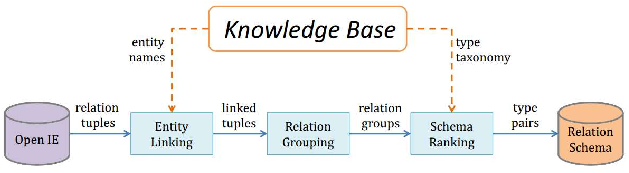
\includegraphics[width=0.9\columnwidth]{figure/tinf/tinf_approach-crop.eps}
    %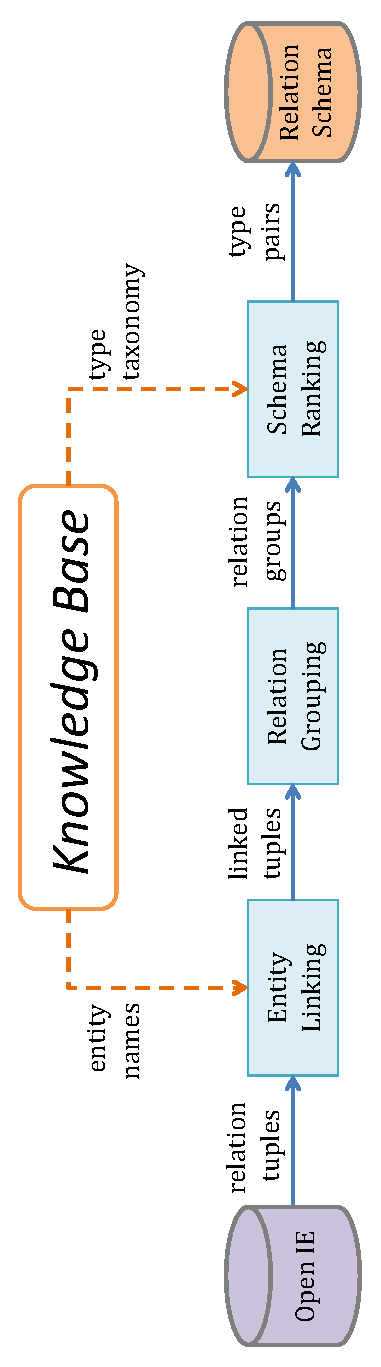
\includegraphics[angle=270,width=\columnwidth]{figure/tinf/system-crop.eps}
    \bicaption{二元关系模式挖掘的流程框图。}{System architecture of type inference of binary relations.}
    \label{fig:tinf-workflow}
\end{figure*}
%\KZ{Redraw this figure as the three boxes in the middle turned out to be
%black in my version of PDF. Also, instead of naming ``ReVerb'' and ``Freebase''
%specifically, use generic terms like ``Open IE'' and ``Taxonomy''. We want
%this system to be general and not tied specifically to ReVerb or Freebase,
%though the actual implementation and eval are on ReVerb and Freebase. These
%we can say in the eval section.}

二元关系模式挖掘的系统架构如\figref{fig:tinf-workflow}所示。
整个系统的输入为开放式信息抽取系统中的所有关系三元组,
经过实体链接、关系分组以及模式排序三个步骤之后,
这些三元组将会转换为一系列排好序的主宾语类型搭配。
每个步骤概括如下,本节将对它们进行具体描述。
%The system takes Open IE relation tuples as the input,
%then performs entity linking, relation grouping and schema ranking
%to translate them into final ranked list of schemas.

% firstly, entity linking (3 sent)
\textbf{(1) 实体链接:}
关系三元组中的参数实体均为字符串形式。
我们通过模糊字符串匹配的方式,将主宾语分别映射到知识库中的不同实体。
%Relation arguments are linked to entities in the knowledge base by
%fuzzy string matching. Each entity in the knowledge base has a unique identifier.

% secondly, relation grouping (2 sent)
\textbf{(2) 关系分组:}
经过链接之后,关系表达形式相近的三元组将聚集在一起,形成一个大的分组。
并且,每一个分组会从内部的不同关系中选择一个,作为整组的代表关系。
%Linked tuples sharing similar relation patterns are grouped together.
%Besides, each group has a representative relation pattern, which is generated from all the patterns within the group.

% thirdly, simultaneously SP (3 sent)
% need to refine at the last sentence.
\textbf{(3) 关系模式排序:}
对分组内的每一个具有链接的关系实例,其主宾语将转换为知识库中对应的类型。
根据不同的类型搭配所覆盖的三元组数量,以及各个类型的宽泛或具体程度,
对所有候选的关系模式进行排序并输出。
%For each linked tuple in one relation group, argument entities are transformed into types drawn from the knowledge base.
%Then this procedure ranks type pairs (schemas) in terms of how much Open IE tuples a type pair can cover and how specific a type concept is.



\subsubsection{实体链接}
\label{sec:tinf-linking}

% 0. what are we going to do ?
% Given a relation tuple, we are going to find representative Freebase entities
% which stand for the arguments.
% 1. Formally definition
在实体链接步骤中,一个关系三元组的主宾语将分别映射到知识库中的实体,
形成带链接的三元组($e_1$, $rel$, $e_2$),并配有对应的链接分值。
%Each entity in Freebase has one or more aliases. The default one is the name of this entity.
%For example, the entity \textit{m.02\_286} has the name ``New York City'' and other aliases
%such as ``The Big Apple'' ``NYC'' and ``Empire City''.
% 4. leverage multiple namees to build an invert index.
由于每一个三元组所具有的信息较少,并没有提供足够的上下文,
因此实体链接过程主要基于主宾语名称以及实体在知识库中名称的模糊匹配。

实体在知识库中存在至多一个标准名称以及多个别名,
例如Freebase中,实体的标准名称和别名分别对应
\textit{type.object.name}以及\textit{common.topic.alias}属性。
我们利用这些属性值构建了从单词指向不同名称的倒排索引,
并进一步生成每个关系参数的候选实体。
% 5. stop word set is used, and use the idf score to weight words.
我们用$alias$表示知识库中的一个名称(或别名),
若将其看做单词的集合(bag-of-words),那么显然单词之间具有不同的重要性。
直观上看,若$alias$中某单词$w$出现在极少数的名称中,那么它对整个名称而言更加重要;
反之类似``of'', ``the'' 等停止词会出现在大多数名称里,那么在模糊匹配的过程中,其权重就很低。
因此我们利用文档频率倒数(Inverted Document Frequency)用于拟合单词$w$的权重:
\begin{equation}
idf(w)=1\ /\log(|\{alias : w \in alias\}|).
\end{equation}
此外,我们直接从知识库的名称中过滤停止词,相当于它们的idf分值为0。
%Besides, stop words are removed from aliases, treating their idf scores as 0.
% 6. matching rule: intersect >= N - 1, weighted overlap score >= threshold
为了衡量关系三元组中的关系参数$arg$与知识库名称$alias$间的模糊匹配程度,
我们计算两者之间的带权重叠分值:
\begin{equation}
overlap(arg, alias) = \frac {\sum\limits_{w \in arg \cap alias} idf(w)} {\sum\limits_{w \in arg \cup alias} idf(w)}.
\end{equation}
对于候选实体$e$,我们分别计算其不同名称与关系参数的模糊匹配分值,
最终选取最高分代表实体$e$与关系参数$arg$的匹配度:
\begin{equation}
sim(e, arg) = \max\limits_{alias \in Alist(e)} overlap(arg, alias).
\end{equation}

% \KQ{TODO: Two Strategies: Just choose the best separately, or FB 2-hop connectable}

为了控制候选实体的质量,
对于由$m$个单词构成的关系参数(停止词忽略不计),
我们仅考虑那些存在至少一个名称具有$m-1$个单词重叠,
同时模糊匹配度高于阈值$\tau$的候选实体。
% we can tune the threshold
% we can use formula to show the weighted score, that is intersect / union, weighed.
% 7. multiple matching, select the one with best wScore.
% 8. tie breaker: count occurrence in freebase relations.
%if there still has a tie, the most popular entity is selected. The popularity of an entity is calculated
%by counting number of relations it has in Freebase.
对于每个关系三元组中的主宾语,我们分别抽取匹配度排名前10的候选实体,用于后续的计算。

对单个关系参数进行匹配计算之后,我们将计算关系三元组
($arg_1$, $rel$, $arg_2$)与实体对($e_1$, $e_2$)之间的联合匹配度。
联合匹配度的定义方式有两种。
第一种匹配方式较为朴素(Naive),仅考虑关系中的两个参数与各自实体的匹配程度,
主宾语实体互相之间并无直接影响:
\begin{equation}
    \label{eqn:naive}
    F(arg_1, e_1, arg_2, e_2, rel) = sim(e_1, arg_1) \cdot sim(e_2, arg_2).
\end{equation}

第二种匹配方式除了考虑$e_1$和$e_2$各自的匹配分数,还考虑到了这两个实体之间存在的联系,
在知识库上体现为连接它们的谓词或谓词序列。
我们以$\vec{w}$表示$rel$的所有单词,
$\vec{p}$表示知识库中连接$e_1$和$e_2$的谓词路径,其长度至多为2。
若实体$e_1$与$e_2$可以通过长度为1的路径相连,
则意味着知识库中存在通过某谓词$p$连接的事实三元组$p(e_1, e_2)$。
类似地,若$e_1$和$e_2$之间通过长度为2的路径相连,
则意味着存在$p_1, p_2$以及中间实体$e'$,
使得事实$p_1(e_1, e')$以及$p_2(e', e_2)$存在于知识库中。
我们利用朴素贝叶斯模型,利用条件概率的形式定义
谓词序列$\vec{p}$与关系$\vec{w}$之间的相关程度:
\begin{equation}
\begin{aligned}
    P(\vec{p}\, |\, \vec{w}) & \approx \prod\nolimits_p P(p\, |\, \vec{w})  \\
                        & \propto \prod\nolimits_p P(p) \prod\nolimits_w P(w\, |\, p).
\end{aligned}
\end{equation}

Yao等人\cite{yao2014information}将知识库谓词序列与关系的对应建模为机器翻译模型,
并根据对齐模型IBM Model 1\cite{brown1993mathematics}学习谓词的先验概率$P(p)$以及
转移概率$P(w|p)$。
基于已有工作的概率模型,给定关系后预测谓词序列的条件概率$P(\vec{p}\, |\, \vec{w})$
便可计算得出。
对于候选实体$e_1$和$e_2$,它们之间的谓词序列与关系$rel$越接近,
则实体链接结果越有可能正确。
因此,我们通过枚举$e_1$和$e_2$之间所有满足长度条件的谓词序列,
计算关系实例与实体对之间的相似度:
\begin{equation}
    \label{eqn:full}
    F(arg_1, e_1, arg_2, e_2, rel) = sim(e_1, arg_1) \cdot
               sim(e_2, arg_2) \cdot
		\sum\nolimits_{\vec{p}} P(\vec{p} | \vec{w}).
\end{equation}

由于条件概率$P(\vec{p} | \vec{w})$的计算涉及到大量连乘,
其数值在不同实体对之间的的差别较为明显,
这也使得其在\eqnref{eqn:full}中具有较高的地位。
而当所有候选实体间的谓词序列与当前关系都不相似的时候,
条件概率的随机波动反而会带来不小的干扰。
因此,我们采用了一种集成(Ensemble)方案:
首先定义条件概率阈值$\rho$,
对于当前关系实例的所有候选实体对,
若其中存在至少一条与关系足够相近的谓词序列,
即满足$P(\vec{p}\, |\, \vec{w}) > \rho$时,
模型使用\eqnref{eqn:full}进行整体匹配度计算,
否则模型退回到\eqnref{eqn:naive},使用朴素的方式寻找最佳实体对。
最后,我们选择分数最高的实体对,作为关系三元组的唯一链接结果。


%\footnote{The popularity of an entity is calculated by counting number of relations it has in the taxonomy.}
%The other strategy (SIM) selects all the $\langle ent1,\ ent2 \rangle$ pairs simultaneously,
%where $ent1$ is reachable from $ent2$ in the taxonomy by 1-hop or 2-hop relation.
%Experimental results on these two strategies are shown in Section 4.


% 9. SUTime is used to map years and datetime.

% check other papers, learn how to introduce FB without too much words.
% 10. discard non-match to guarantee accuracy of linking.
% If one argument fails to link to any entity, the corresponding relation tuple is discarded.
% Ranking Method May Change?
%   use wScore threshold to filter entities
%   then sorting by interLen, then popularity ??? (maybe we can have a try afterwards)
%


%\begin{table}[htbp]
%	\centering
%	\caption{Syntactic Transform Rules}
%	\begin{tabular}{|l|l|}
%		%\toprule
%        \whline
%		Category & Pattern Template \\
%		%\midrule
%        \hline
%        % Continuous Tense & \{$adv_1$\} \textbf{be} \{$adv_2$\} verb:VBG \{text\}
%        %                  & $verb_{lem}$ \{phrase\} \\
%		% Participle Tense & \{$adv_1$\} \textbf{have} \{$adv_2$\} verb:VBN \{text\}
%        %                  & $verb_{lem}$ \{phrase\} \\
%        % Participle + Passive & \{$adv_1$\} \textbf{have} \{$adv_2$\} been \{text\}
%        %                      & is \{text\} \\
%        Continuous Tense & \textbf{be} verb:VBG \{phrase\} \\
%		Participle Tense & \textbf{have} verb:VBN \{text\} \\
%        Future Tense & \textbf{will}/\textbf{shall} verb:VB \{pharse\} \\
%                     & \textbf{be} going to verb:VB \{phrase\} \\
%		%\bottomrule
%        \whline
%	\end{tabular}%
%	\label{tab:synt rules}%
%\end{table}




\subsubsection{关系分组}
% 8 sents.
% 1. group tuples together, give definition
%A relation group consists of linked tuples sharing similar relation patterns,
%along with a representative pattern.
% 2. same & syntactically similar rel. patterns will be in a group, no overlapping.
%Each linked tuple belongs to one unique group.

这个步骤对所有已链接的关系三元组进行聚类,拥有相似关系描述的三元组将归为同一分组。
每个三元组仅存在于唯一一个分组中。

% 3. algorithm: syntactic rules to convert tense,
% mainly focus on 3 tense: will/should/must be, be -ing, participle

%We define syntactically equivalence between two relation patterns, as both of them can be converted
%into the same simple pattern by a list of transformations.
%Every relation pattern in one group is equivalent with each other.
这个步骤的思路是通过语法转换,将复杂的关系描述进行简化。
如果两个不同的关系具有相同的简化形式,那么视为其语义相同,并归为同一分组。
首先考虑到形容词、副词以及情态动词的存在与否,
基本上不会改变一个关系中主宾语实体所属的类型,
因此我们将这些词从关系描述中移除。
此外,大多数关系包含动词,但时态并不一致,
因此我们将所有时态统一为现在时。
此外,关系中的被动语态将会被保留,不做形式转变。
% 4. Create a table, showing the rules to find them.
%The detail of syntactic rules is shown in Table 1.
%\KQ{refer to Liang et al., 2014 to build the rule table, containing continuous, participle, be-the-name-of
%and passive form}
% For example, a --> b
% check liang's 14 paper to learn the representation of tables.
% 5. use stanford parser to tokenize & postag.
% 6. representative relation: present tense
例如经过语法转换之后,下列关系实例将归为同一组:
(X, \textit{resign from}, Y), (X, \textit{had resigned from}, Y)
以及(X, \textit{finally resignd from}, Y)。
最后,每一个分组的代表关系为组内关系的统一简化形式。
如上例所示,三个关系实例属于\textit{``resign from''}组。


\subsubsection{类型搭配排序}
\label{sec:tinf-approach-sort}

给定一个关系分组$r$,这一步骤将生成排好序的主宾语类型对,即该关系的代表性模式。
以二元关系 ``play in'' 举例,理想情况下,生成的结果里会包含模式
$\langle actor,\ film \rangle$以及$\langle pro\_athlete,\ sports\_league \rangle$。

对于带链接的三元组($e_1$, $rel$, $e_2$),
若在知识库中,$e_1$具有类型$t_1$,而$e_2$具有类型$t_2$,
那么该三元组为类型搭配 $\langle t_1,\ t_2 \rangle$ 的一个支持实例。
一个实体有可能从属于多种类型,无论类型宽泛或具体,因此一个三元组可以支持多种类型搭配。
对关系分组$r$中的所有实例进行处理,我们可以得到每一种类型搭配
所对应的支持集合:
\begin{equation}
sup_{r}(\langle t_1, t_2 \rangle) = \{ \langle e_1, e_2 \rangle\ |\ (e_1, t_1) \in IsA,\; (e_2, t_2) \in IsA \}.
\end{equation}

得到所有可能的类型搭配之后,我们可以根据支持集合的大小进行排序。
由于每个实体从属于多种类型,因此显然更加宽泛的类型搭配通常会被排在前列。
但是,对于人类或是机器理解一个自然语言关系,宽泛的关系模式所具有的信息量相对不足,
尤其是当两种类型对具有几乎一致的支持集合时,往往更具体的类型对具有更好的代表性。
例如对于关系 ``\textit{X die in Y}'' ,
在开放式信息抽取和实体链接均不产生错误的情况下,
类型对$\langle person,\ location \rangle$和
$\langle deceased\_person,\ location \rangle$将对应完全一致的支持集合。
后者对关系的描述更加具体,在不丢失支持实例的同时,尽可能缩小主语在知识库中的范围。

由此可见,对候选类型对的排序需要考虑每个类型的相对粒度。
接下来的目标就是提取知识库中类型之间的包含关系,建立更加完整的层次结构。
我们定义所有属于类型$t$的实体为
$cover(t) = \{e\; |\; (e, t) \in IsA\}$。
理想情况中,若$t_1$包含于$t_2$,
那么所有$t_1$中的实体都从属于$t_2$,
即$cover(t_1) \subseteq cover(t_2)$.
这样的包含规则称为 ``{严格类型包含}'' 。
例如在Freebase中,类型\textit{person}所包含的其它类型包括
\textit{actor},\textit{politician}以及\textit{deceased\_person}等。

然而,严格类型包含在知识库中并不多见,
主要原因是知识库的类型定义和人类对自然界的归纳存在一定差别,
以Freebase中的\textit{award\_winner}为例,
类型中绝大多数实体都为自然人,但依然包含少量的组织实体在内。
基于严格类型包含的规则,
\textit{award\_winner}与\textit{person}之间毫无包含关系,
但事实上,考虑到非自然人实体仅存在极少数,
两个类别之间在很大程度上依然构成从属关系。
另一方面,由于实体的类型涉及到人工标记,一旦出现类型标记错误,
就有可能导致类型之间无法满足严格包含条件。


为了能更好地建立类型层次关系,我们使用一种更加松弛的类型包含定义方式。
具体而言,若$t_1$中足够数量的实体从属于$t_2$,那么就认为包含关系成立。
因此,我们定义$t_1$包含于$t_2$的度,即对应实体包含的比例:
\begin{equation}
deg(t_1 \subseteq t_2) = \frac{\left|cover(t_1) \cap cover(t_2)\right|} {\left|cover(t_1)\right|}.
\end{equation}
%$deg(Supp_1\subseteq Supp_2)=\left|Supp_1 \cap Supp_2\right| / \left|Supp_1\right|$.
若$deg(t_1 \subseteq t_2) > \epsilon$,
则$t_1$包含于$t_2$。
阈值$\epsilon$表示松弛程度,若$\epsilon=1$,则松弛包含退化为严格包含。
若$\epsilon$太小,那么类型之间将具有非常丰富的层次关系,
但其有效性则会下降。
最后,遍历知识库中所有的类型,我们就可以得到特定松弛程度下的类型层次图。
%\figref{fig:tinf-taxonomy}展示了Freebase中的一部分类型之间的层次关系,
%用不同样式的边表示不同松弛程度的包含。
%TODO: taxonomy弄一个好一点的图,可以撑1/3页呢。

随着类型层次关系建立完毕,我们就可以定义不同类型搭配之间的包含关系。
若类型对$\langle t_1,\ t_2\rangle$被另一个类型对
$\langle t_3,\ t_4\rangle$,则意味着以下条件之一成立:
i) $t_1 \subseteq t_3$,$t_2 \subseteq t_4$;
ii) $t_1 \subseteq t_3$,$t_2 = t_4$;
iii) $t_2 \subseteq t_4$,$t_1 = t_3$。
最终的类型对排名体现为支持集合大小和类型对包含关系的共同作用。
以支持集合降序排列为基础,
若类型对$tp=\langle t_1, t_2 \rangle$包含于另一个类型对$tp'$,
且各自的支持集合大小($|sup_{r}(tp)|$)几乎一致,
那么$tp'$将排在$tp$之前。
我们同样可以根据重叠关系实例的覆盖程度,
来定义两个支持集合是否几乎一致:
\begin{equation}
\frac{\left|sup_{r}(tp)\right|-\left|sup_{r}(tp')\right|} {max(\left|sup_{r}(tp)\right|,\ \left|sup_{r}(tp')\right|)} < \lambda,
\end{equation}
其中$\lambda$为判断集合中的元素是否一致的阈值。


%# -*- coding: utf-8-unix -*-
% !TEX program = xelatex
% !TEX root = ../thesis.tex
% !TEX encoding = UTF-8 Unicode

% how to evaluate?
% random picking relation, labeling true or false?
% the count precision@x?

% check: 1. GY's paper
%        2. ritter's paper

% Check their page size
% write about our size.
% and compare the version of MI-Equal, MI-Uniform, TfIdf-Equal, TfIdf-Uniform
%%In the demonstration part, we first introduce the experimental setup.
%%Secondly we evaluate the accuracy of relation type inferring.
%%Then we present our web interface of RvSp system, and finally
%%we provide some example relations with the inferred argument types.

\subsection{实验}
\label{sec:tinf-exp}
% Add Freebase dump citation
%\KZ{First, say a bit about the ReVerb dataset, and the specifics of
%Freebase. Then say something about our implementation details in the
%3 steps, such as parser we used, etc. What about the numbers in the table?}

\subsubsection{实验设置}
我们在实验中使用的知识库为Freebase\cite{bollacker2008freebase}在2014年2月16日的版本,
包含了大约40,000,000个不同实体,以及1,700个主要类型。
%\footnote{Freebase的每个类型都对应一个id,例如``professional athlete''
%在知识库中的类型id为$sports.pro\_athlete$。}。
实验中使用的开放式信息抽取系统为ReVerb\cite{fader2011identifying},
ReVerb数据集提供了多种版本,我们使用的版本包含了置信度最高的14,000,000个关系三元组。
%Each entity belongs to at least one type.
%When compared with other knowledge bases, Freebase has a much greater focus on named entities than {\tt WordNet}.
%Besides, the type hierarchy of {\tt Yago} is too fine-grained, which is not suitable for schema inferring.
%Considering aspects mentioned above, we adapt Freebase as our knowledge base in our work.
%The input ReVerb dataset is released by Lin et al.\shortcite{lin2012entity}, containing 3 millions of relation tuples with high quality.

ReVerb抽取的三元组中,部分关系参数无法链接到Freebase中的某一个实体,
例如三元组($Metro\ Manila,\ consists\ of,\ \textbf{12 cities}$),
其宾语显然不是一个实体,而是用自然语言描述的类型。
这部分三元组不是我们的研究对象,需要进行过滤。
考虑到在自然语言中,概念通常对应非专有单词,并且多为小写,
因此我们根据WordNet收集了常用的非专有单词。
若一个三元组中包含纯小写,或纯粹由非专有单词构成的主宾语,
那么该三元组将被过滤。
除此之外,ReVerb三元组中还具有时间或日期作为关系参数的情况,
例如 ``Jan. 16th, 1981'' 作为宾语,但同样不对应Freebase的某个实体。
为应对这种情况,我们使用SUTime\cite{chang2012sutime}工具识别
时间或日期,将它们替换为具有$type.datetime$类型的虚拟实体。
经过清理之后,系统共收集了3,234,208个三元组,
对应171,168个不同的关系分组。

% Talk about entity linking.
%We make the following parameter settings by empirics:
%The following parameters are tuned using a development set:
实验中具体使用的参数值为:
$\tau = 0.667$,$\rho = e^{-50}$,
$\epsilon=0.6$以及$\lambda = 5\%$。
关系分组步骤中,我们使用Stanford Parser\cite{klein2003accurate}
对每个关系进行词性标注、语法分析以及时态转换。
%All the data sets involved in the evaluation are available at
%\url{http://202.120.38.146/schema/}.



\subsubsection{结果分析}
我们首先对实体链接进行评测。
由于ReVerb没有提供主宾语的链接结果,
我们从所有关系实例中随机挑选200个三元组,并人工标注这些主宾语所链接的实体。
我们对比实体链接过程的朴素方法和集成方法,
使用准确率(Precision),召回率(Recall),$F_1$分值,以及MRR\cite{liu2009learning}
作为评价指标。
MRR为平均排名倒数(Mean Reciprocal Rank),
即统计正确的链接结果在输出列表中的排名,再计算所有三元组上排名倒数值的平均。
当一个三元组的主宾语均链接正确时,我们才认为该三元组链接正确。
实验结果比较如\tabref{tab:tinf-linking}所示。
不同于常规文本的实体链接,由于每个三元组的上下文极少,链接具有一定难度。
基于集成的链接方法引入了关系与实体间语义的匹配模型,
使主宾语的链接实体互相影响,
链接过程的准确率和召回率均得到稳定提升。

%We assigned 3 human annotators to judge whether both arguments are linked to correct entities.
%We don't have a gold set for entity linking, but we assume that each unlinked relation tuple corresponds to a linked tuple.
%Therefore, we can approximate the recall of entity linking as:
%\begin{equation}
%recall\ =\ \frac {precision * \#Linked\ Tuples} {\#Relation\ Tuples}
%\end{equation}
%For each strategy, the total number of linked tuples, precision, recall and F1 are listed in \tabref{tab:linking_result}.

\begin{table}[ht]
	\centering
	\bicaption{ReVerb三元组的实体链接实验结果。}{Entity linking result.}
	\begin{tabular}{c|cccc}
		%\toprule
        \hline
	    Linking Strategy & Precision & Recall & $F_1$ & MRR \\
        \hline
        Naive    & 0.371 & 0.327 & 0.348 & 0.377 \\
        Ensemble & 0.386 & 0.340 & 0.361 & 0.381 \\
        \hline
	\end{tabular}%
	\label{tab:tinf-linking}%
\end{table}


接下来我们衡量二元关系的主宾语搭配结果,主要关注具有较多实例的关系分组。
我们首先从包含至少500个三元组的关系分组中,随机选择50个分组,
对于每个分组,我们挑选出支持集合数量最大的100个类型对作为评测的对象。
我们将这些类型对分配给3位对Freebase类型有了解的标注者,
每个标注者根据自己的理解,判断类型对是否适合于描述对应关系,
并标注0到3的分值。
将三位标注者的打分进行平均,即可得到这50个关系分组的类型对排序。

我们使用点对点互信息(Pointwise Mutual Information)\cite{church1990word}
作为基线模型,该模型在选择偏好任务中被使用,例如文献\parencite{resnik1996selectional}。
PMI模型使用以下公式定义一个关系$r$与类型对$tp$的关联度:
\begin{equation}
PMI(r, tp) = p(r, tp) \log \frac {p(r, tp)}{p(r, *) p(*, tp)},
\end{equation}
其中$p(r, tp)$代表联合概率,即关系分组为$r$,且支持$tp$的三元组占所有三元组的比重,
$*$代表任意关系或类型对。

我们使用MRR分数进行评测,衡量不同方法生成的最佳关系模式在标注列表中的位置。
如\tabref{tab:tinf-mrr}所示,和基线模型进行比较,
我们的方法在MRR指标上获得了10.1\%的相对提升。

\begin{table}[ht]
	\centering
	\bicaption{二元关系模式推理的评测结果。}{End-to-end schema inference results.}
	\begin{tabular}{c|c}
        \hline
		Approach & MRR Score \\
        \hline
        PMI Baseline & 0.306 \\
        Our Approach & 0.337 \\
        \hline
	\end{tabular}%
	\label{tab:tinf-mrr}%
\end{table}

%\begin{figure%}[htp]
%\centering \scalebox{0.6}{\includegraphics{eval.eps}}
%%\epsfig{file=figure1-cropped.eps, width=2\columnwidth}
%%\scalebox{0.35}
%\caption{Average precision at different ranks.}
%\label{fig:precision}
%\end{figure}

% We randomly sample K relations, use 3 annotators to annotate whether a type pair is true or not.
% count precision@px

%\subsection{Web Interface}
%In addition, we set up a website \footnote{http://202.120.38.146/rvsp} for users to query the schemas of a binary relation.
%Users can search for type pairs by providing the binary relation alone, or the relation with the type of either arg1 or arg2.
%The interface will output the ranked list of schemas satisfying the input constraint along with its support instances.
%Before querying, the interface will transform the relation pattern, using the method introduced in section 4.

%Due to argument types in RvSp is recognized by Feebase type id, which doesn't match its name exactly, we provide typing suggestion in the web interface, %making users easily enter Freebase types.
%Users can browse Freebase website \footnote{http://www.freebase.com} for detail information about type id.

%
%\\
%\\
%
%\begin{figure}[ht]
%\centering
%\epsfig{file=cropped-demo1.eps, width=0.6\columnwidth, angle=270}
%\caption{Query Interface}
%\label{fig:demo1}
%\end{figure}
%
%
%\figref{fig:demo1} shows the result page.
%User can click ``page up'' and ``page down'' to check more results.
%Besides, for each relation schema, user can click ``detail'' link too check all its support tuples.
%The schema details are shown in \figref{fig:demo2}.
%\\
%\\
%
%\begin{figure}[ht]
%\centering
%\epsfig{file=cropped-demo2.eps, width=0.6\columnwidth, angle=270}
%\caption{Schema Details}
%\label{fig:demo2}
%\end{figure}
%

最后,\tabref{tab:tinf-sample}列举了一些具体的关系分组,
以及我们系统抽取的关系模式。
我们可以看出,当构建了Freebase的类型层次结构之后,
系统能够同时得到粗粒度和细粒度的类型信息,
因此最终生成的类型对具有更加丰富的信息量。


%
%\begin{table*}[htbp]
%	\centering
%	\caption{Sample Relation Schemas}
%	\begin{tabular}{Ic|l|lI}
%		%\toprule
%        \whline
%		Relation & Arg1 Type & Arg2 Type \\
%        \whline
%        & book.author & book.book \\
%        & book.author & book.written\_work \\
%        be the writer of & tv.tv\_writer & award.award\_nominated\_work \\
%        & people.person & book.book \\
%        & people.person & book.written\_work  \\
%        \hline
%        & fictional\_universe.fictional\_character & tv.tv\_actor  \\
%        & fictional\_universe.fictional\_character & film.actor  \\
%        be play by & fictional\_universe.fictional\_character & people.person  \\
%        & fictional\_universe.fictional\_character & influence.influence\_node  \\
%        & people.person & tv.tv\_actor  \\
%        \hline
%        & organization.organization\_founder & organization, organization \\
%        & people.person & organization, organization \\
%        found & people.deceased\_person & organization, organization \\
%        & organization.organization\_founder & business.business\_operation \\
%        & organization.organization\_founder & business.employer \\
%        \whline
%	\end{tabular}%
%	\label{tab:sample_relation}%
%\end{table*}
\begin{table}[ht]
	\centering
	\bicaption{生成的二元关系模式举例。}{Real examples of generated relation schemas.}
	\begin{tabular}{c|c}
        \hline
		Relation & Top-3 schemas \\
        \hline
        & $\langle location,\ location \rangle$ \\
        be found at & $\langle employer,\ location \rangle$ \\
        & $\langle organization,\ location \rangle$\\
        \hline
        & $\langle person,\ tv\ program \rangle$\\
        appear on & $\langle person,\ nominated\_work \rangle$\\
        & $\langle person,\ winning\ work \rangle$\\
        \hline
        & $\langle person,\ nominated\_work \rangle$\\
        be the writer of & $\langle person,\ film \rangle$\\
        & $\langle person,\ book\_subject \rangle$\\
        \hline
	\end{tabular}%
	\label{tab:tinf-sample}%
\end{table}



%============================================================%

\section{小结}
% what did we do
In summary, our work describes a data driven approach of
relation schema inference.
By maximizing the support of both arguments simultaneously,
our system is able to generate human-readable type pairs for 
a binary relation from Open IE systems. 
% what is the result
Our experiments shows that the top ranked relation schemas for 
each relation are accurate according to human judges.
The proposed framework can be integrated with future Open IE systems.
% what's the future vision
%In the future, we are going to explore researches on question answering field, leveraging these
%type pair information to improve answer quality.


本章的研究成果已发表于2015年国际会议Empirical Methods in Natural Language Processing
(EMNLP-2015),论文题目为
``Inferring Binary Relation Schemas for Open Information Extraction''。
